\pdfinfoomitdate=1
\pdftrailerid{}
\pdfsuppressptexinfo=-1
\documentclass[border=6pt]{standalone}
\usepackage{amsmath,amssymb}
\usepackage{tikz}
\usetikzlibrary{arrows.meta,decorations.pathreplacing,positioning}
\begin{document}
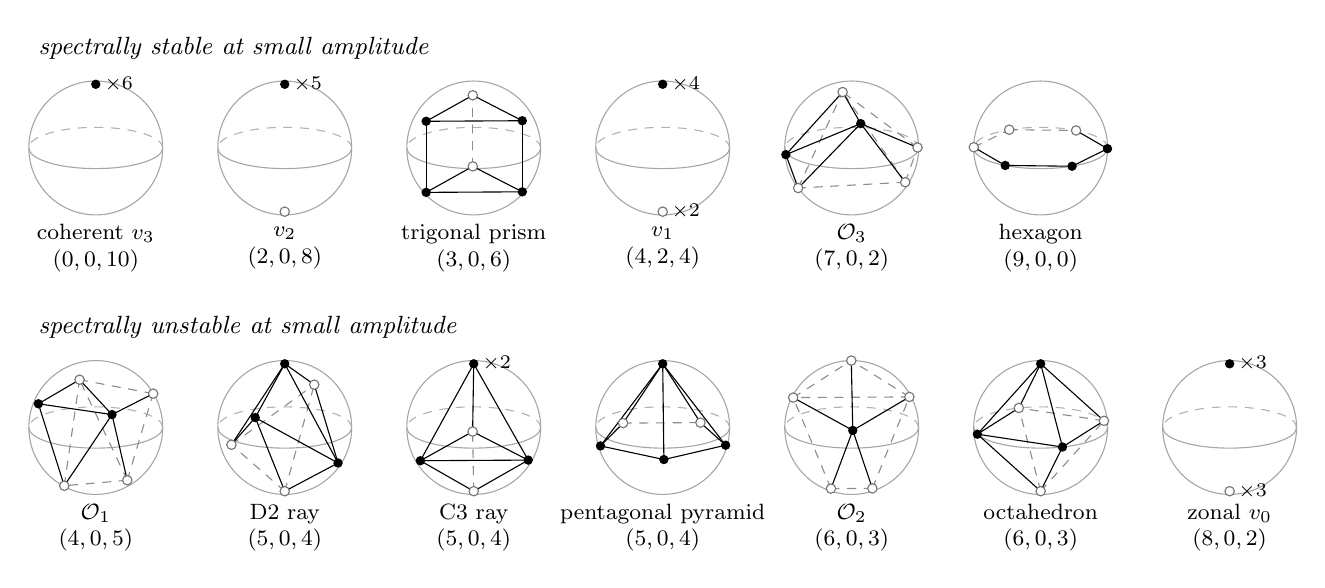
\begin{tikzpicture}[line cap=round]
\node[font=\small\itshape, anchor=west] at (-0.85,1.27) {spectrally stable at small amplitude};
\draw[black!35] (0.000,0.000) circle (0.850);
\draw[black!30, dashed] (0.850,0.000) arc[start angle=0, end angle=180, x radius=0.850, y radius=0.262];
\draw[black!35] (0.850,0.000) arc[start angle=0, end angle=-180, x radius=0.850, y radius=0.262];
\fill (0.000,0.809) circle (1.7pt);
\node[font=\scriptsize, anchor=west, inner sep=1pt] at (0.070,0.809) {$\times 6$};
\node[font=\footnotesize, align=center] at (0.000,-1.270) {coherent $v_3$\\ $(0, 0, 10)$};
\draw[black!35] (2.400,0.000) circle (0.850);
\draw[black!30, dashed] (3.250,0.000) arc[start angle=0, end angle=180, x radius=0.850, y radius=0.262];
\draw[black!35] (3.250,0.000) arc[start angle=0, end angle=-180, x radius=0.850, y radius=0.262];
\draw[black!55, fill=white] (2.400,-0.809) circle (1.7pt);
\fill (2.400,0.809) circle (1.7pt);
\node[font=\scriptsize, anchor=west, inner sep=1pt] at (2.470,0.809) {$\times 5$};
\node[font=\footnotesize, align=center] at (2.400,-1.270) {$v_2$\\ $(2, 0, 8)$};
\draw[black!35] (4.800,0.000) circle (0.850);
\draw[black!30, dashed] (5.650,0.000) arc[start angle=0, end angle=180, x radius=0.850, y radius=0.262];
\draw[black!35] (5.650,0.000) arc[start angle=0, end angle=-180, x radius=0.850, y radius=0.262];
\draw[black!45, dashed, thin] (4.788,-0.234) -- (4.788,0.669);
\draw[black, thin] (4.196,-0.564) -- (5.417,-0.557);
\draw[black, thin] (4.196,-0.564) -- (4.788,-0.234);
\draw[black, thin] (5.417,-0.557) -- (4.788,-0.234);
\draw[black, thin] (5.417,0.346) -- (4.788,0.669);
\draw[black, thin] (4.196,0.339) -- (5.417,0.346);
\draw[black, thin] (4.196,0.339) -- (4.788,0.669);
\draw[black, thin] (4.196,-0.564) -- (4.196,0.339);
\draw[black, thin] (5.417,-0.557) -- (5.417,0.346);
\fill (4.196,-0.564) circle (1.7pt);
\fill (5.417,-0.557) circle (1.7pt);
\draw[black!55, fill=white] (4.788,-0.234) circle (1.7pt);
\fill (4.196,0.339) circle (1.7pt);
\fill (5.417,0.346) circle (1.7pt);
\draw[black!55, fill=white] (4.788,0.669) circle (1.7pt);
\node[font=\footnotesize, align=center] at (4.800,-1.270) {trigonal prism\\ $(3, 0, 6)$};
\draw[black!35] (7.200,0.000) circle (0.850);
\draw[black!30, dashed] (8.050,0.000) arc[start angle=0, end angle=180, x radius=0.850, y radius=0.262];
\draw[black!35] (8.050,0.000) arc[start angle=0, end angle=-180, x radius=0.850, y radius=0.262];
\draw[black!55, fill=white] (7.200,-0.809) circle (1.7pt);
\node[font=\scriptsize, anchor=west, inner sep=1pt] at (7.270,-0.809) {$\times 2$};
\fill (7.200,0.809) circle (1.7pt);
\node[font=\scriptsize, anchor=west, inner sep=1pt] at (7.270,0.809) {$\times 4$};
\node[font=\footnotesize, align=center] at (7.200,-1.270) {$v_1$\\ $(4, 2, 4)$};
\draw[black!35] (9.600,0.000) circle (0.850);
\draw[black!30, dashed] (10.450,0.000) arc[start angle=0, end angle=180, x radius=0.850, y radius=0.262];
\draw[black!35] (10.450,0.000) arc[start angle=0, end angle=-180, x radius=0.850, y radius=0.262];
\draw[black!45, dashed, thin] (10.436,0.006) -- (9.485,0.710);
\draw[black!45, dashed, thin] (10.280,-0.435) -- (10.436,0.006);
\draw[black!45, dashed, thin] (10.280,-0.435) -- (9.485,0.710);
\draw[black!45, dashed, thin] (10.280,-0.435) -- (8.920,-0.509);
\draw[black!45, dashed, thin] (8.920,-0.509) -- (9.485,0.710);
\draw[black, thin] (9.485,0.710) -- (9.715,0.309);
\draw[black, thin] (8.764,-0.085) -- (9.715,0.309);
\draw[black, thin] (8.764,-0.085) -- (9.485,0.710);
\draw[black, thin] (10.436,0.006) -- (9.715,0.309);
\draw[black, thin] (10.280,-0.435) -- (9.715,0.309);
\draw[black, thin] (8.920,-0.509) -- (9.715,0.309);
\draw[black, thin] (8.920,-0.509) -- (8.764,-0.085);
\draw[black!55, fill=white] (10.280,-0.435) circle (1.7pt);
\draw[black!55, fill=white] (8.920,-0.509) circle (1.7pt);
\fill (8.764,-0.085) circle (1.7pt);
\draw[black!55, fill=white] (10.436,0.006) circle (1.7pt);
\draw[black!55, fill=white] (9.485,0.710) circle (1.7pt);
\fill (9.715,0.309) circle (1.7pt);
\node[font=\footnotesize, align=center] at (9.600,-1.270) {$\mathcal{O}_3$\\ $(7, 0, 2)$};
\draw[black!35] (12.000,0.000) circle (0.850);
\draw[black!30, dashed] (12.850,0.000) arc[start angle=0, end angle=180, x radius=0.850, y radius=0.262];
\draw[black!35] (12.850,0.000) arc[start angle=0, end angle=-180, x radius=0.850, y radius=0.262];
\draw[black!45, dashed, thin] (11.151,0.009) -- (11.601,0.232);
\draw[black!45, dashed, thin] (11.601,0.232) -- (12.450,0.222);
\draw[black, thin] (12.450,0.222) -- (12.849,-0.009);
\draw[black, thin] (12.849,-0.009) -- (12.399,-0.232);
\draw[black, thin] (12.399,-0.232) -- (11.550,-0.222);
\draw[black, thin] (11.550,-0.222) -- (11.151,0.009);
\fill (11.550,-0.222) circle (1.7pt);
\draw[black!55, fill=white] (11.151,0.009) circle (1.7pt);
\fill (12.399,-0.232) circle (1.7pt);
\draw[black!55, fill=white] (11.601,0.232) circle (1.7pt);
\fill (12.849,-0.009) circle (1.7pt);
\draw[black!55, fill=white] (12.450,0.222) circle (1.7pt);
\node[font=\footnotesize, align=center] at (12.000,-1.270) {hexagon\\ $(9, 0, 0)$};
\node[font=\small\itshape, anchor=west] at (-0.85,-2.28) {spectrally unstable at small amplitude};
\draw[black!35] (0.000,-3.550) circle (0.850);
\draw[black!30, dashed] (0.850,-3.550) arc[start angle=0, end angle=180, x radius=0.850, y radius=0.262];
\draw[black!35] (0.850,-3.550) arc[start angle=0, end angle=-180, x radius=0.850, y radius=0.262];
\draw[black!45, dashed, thin] (0.400,-4.220) -- (0.729,-3.120);
\draw[black!45, dashed, thin] (0.400,-4.220) -- (-0.400,-4.290);
\draw[black!45, dashed, thin] (-0.206,-2.943) -- (0.729,-3.120);
\draw[black!45, dashed, thin] (0.400,-4.220) -- (-0.206,-2.943);
\draw[black!45, dashed, thin] (-0.400,-4.290) -- (-0.206,-2.943);
\draw[black, thin] (0.400,-4.220) -- (0.206,-3.386);
\draw[black, thin] (0.729,-3.120) -- (0.206,-3.386);
\draw[black, thin] (-0.400,-4.290) -- (0.206,-3.386);
\draw[black, thin] (-0.729,-3.249) -- (0.206,-3.386);
\draw[black, thin] (-0.400,-4.290) -- (-0.729,-3.249);
\draw[black, thin] (-0.206,-2.943) -- (0.206,-3.386);
\draw[black, thin] (-0.206,-2.943) -- (-0.729,-3.249);
\draw[black!55, fill=white] (0.400,-4.220) circle (1.7pt);
\draw[black!55, fill=white] (-0.400,-4.290) circle (1.7pt);
\draw[black!55, fill=white] (-0.206,-2.943) circle (1.7pt);
\draw[black!55, fill=white] (0.729,-3.120) circle (1.7pt);
\fill (-0.729,-3.249) circle (1.7pt);
\fill (0.206,-3.386) circle (1.7pt);
\node[font=\footnotesize, align=center] at (0.000,-4.820) {$\mathcal{O}_1$\\ $(4, 0, 5)$};
\draw[black!35] (2.400,-3.550) circle (0.850);
\draw[black!30, dashed] (3.250,-3.550) arc[start angle=0, end angle=180, x radius=0.850, y radius=0.262];
\draw[black!35] (3.250,-3.550) arc[start angle=0, end angle=-180, x radius=0.850, y radius=0.262];
\draw[black!45, dashed, thin] (2.400,-4.359) -- (2.775,-3.006);
\draw[black!45, dashed, thin] (1.723,-3.769) -- (2.775,-3.006);
\draw[black!45, dashed, thin] (2.400,-4.359) -- (1.723,-3.769);
\draw[black, thin] (2.400,-4.359) -- (2.025,-3.424);
\draw[black, thin] (1.723,-3.769) -- (2.025,-3.424);
\draw[black, thin] (2.400,-4.359) -- (3.077,-4.001);
\draw[black, thin] (3.077,-4.001) -- (2.775,-3.006);
\draw[black, thin] (3.077,-4.001) -- (2.025,-3.424);
\draw[black, thin] (2.775,-3.006) -- (2.400,-2.741);
\draw[black, thin] (1.723,-3.769) -- (2.400,-2.741);
\draw[black, thin] (2.025,-3.424) -- (2.400,-2.741);
\draw[black, thin] (3.077,-4.001) -- (2.400,-2.741);
\draw[black!55, fill=white] (2.400,-4.359) circle (1.7pt);
\fill (3.077,-4.001) circle (1.7pt);
\draw[black!55, fill=white] (1.723,-3.769) circle (1.7pt);
\draw[black!55, fill=white] (2.775,-3.006) circle (1.7pt);
\fill (2.025,-3.424) circle (1.7pt);
\fill (2.400,-2.741) circle (1.7pt);
\node[font=\footnotesize, align=center] at (2.400,-4.820) {D2 ray\\ $(5, 0, 4)$};
\draw[black!35] (4.800,-3.550) circle (0.850);
\draw[black!30, dashed] (5.650,-3.550) arc[start angle=0, end angle=180, x radius=0.850, y radius=0.262];
\draw[black!35] (5.650,-3.550) arc[start angle=0, end angle=-180, x radius=0.850, y radius=0.262];
\draw[black!45, dashed, thin] (4.800,-4.359) -- (4.786,-3.602);
\draw[black, thin] (4.786,-3.602) -- (4.800,-2.741);
\draw[black, thin] (4.122,-3.972) -- (4.786,-3.602);
\draw[black, thin] (4.122,-3.972) -- (4.800,-2.741);
\draw[black, thin] (5.492,-3.964) -- (4.800,-2.741);
\draw[black, thin] (4.122,-3.972) -- (5.492,-3.964);
\draw[black, thin] (4.786,-3.602) -- (5.492,-3.964);
\draw[black, thin] (4.800,-4.359) -- (4.122,-3.972);
\draw[black, thin] (4.800,-4.359) -- (5.492,-3.964);
\draw[black!55, fill=white] (4.800,-4.359) circle (1.7pt);
\fill (4.122,-3.972) circle (1.7pt);
\draw[black!55, fill=white] (4.786,-3.602) circle (1.7pt);
\fill (5.492,-3.964) circle (1.7pt);
\fill (4.800,-2.741) circle (1.7pt);
\node[font=\scriptsize, anchor=west, inner sep=1pt] at (4.870,-2.741) {$\times 2$};
\node[font=\footnotesize, align=center] at (4.800,-4.820) {C3 ray\\ $(5, 0, 4)$};
\draw[black!35] (7.200,-3.550) circle (0.850);
\draw[black!30, dashed] (8.050,-3.550) arc[start angle=0, end angle=180, x radius=0.850, y radius=0.262];
\draw[black!35] (8.050,-3.550) arc[start angle=0, end angle=-180, x radius=0.850, y radius=0.262];
\draw[black!45, dashed, thin] (6.697,-3.494) -- (7.679,-3.488);
\draw[black, thin] (6.697,-3.494) -- (7.200,-2.741);
\draw[black, thin] (6.410,-3.784) -- (6.697,-3.494);
\draw[black, thin] (6.410,-3.784) -- (7.200,-2.741);
\draw[black, thin] (7.215,-3.957) -- (7.200,-2.741);
\draw[black, thin] (6.410,-3.784) -- (7.215,-3.957);
\draw[black, thin] (7.999,-3.775) -- (7.200,-2.741);
\draw[black, thin] (7.215,-3.957) -- (7.999,-3.775);
\draw[black, thin] (7.679,-3.488) -- (7.200,-2.741);
\draw[black, thin] (7.999,-3.775) -- (7.679,-3.488);
\fill (6.410,-3.784) circle (1.7pt);
\fill (7.215,-3.957) circle (1.7pt);
\draw[black!55, fill=white] (6.697,-3.494) circle (1.7pt);
\fill (7.999,-3.775) circle (1.7pt);
\draw[black!55, fill=white] (7.679,-3.488) circle (1.7pt);
\fill (7.200,-2.741) circle (1.7pt);
\node[font=\footnotesize, align=center] at (7.200,-4.820) {pentagonal pyramid\\ $(5, 0, 4)$};
\draw[black!35] (9.600,-3.550) circle (0.850);
\draw[black!30, dashed] (10.450,-3.550) arc[start angle=0, end angle=180, x radius=0.850, y radius=0.262];
\draw[black!35] (10.450,-3.550) arc[start angle=0, end angle=-180, x radius=0.850, y radius=0.262];
\draw[black!45, dashed, thin] (9.863,-4.323) -- (10.333,-3.162);
\draw[black!45, dashed, thin] (10.333,-3.162) -- (9.595,-2.700);
\draw[black!45, dashed, thin] (8.857,-3.170) -- (9.595,-2.700);
\draw[black!45, dashed, thin] (10.333,-3.162) -- (8.857,-3.170);
\draw[black!45, dashed, thin] (9.337,-4.326) -- (8.857,-3.170);
\draw[black!45, dashed, thin] (9.863,-4.323) -- (9.337,-4.326);
\draw[black, thin] (9.614,-3.587) -- (10.333,-3.162);
\draw[black, thin] (9.863,-4.323) -- (9.614,-3.587);
\draw[black, thin] (9.614,-3.587) -- (9.595,-2.700);
\draw[black, thin] (9.614,-3.587) -- (8.857,-3.170);
\draw[black, thin] (9.337,-4.326) -- (9.614,-3.587);
\draw[black!55, fill=white] (9.863,-4.323) circle (1.7pt);
\draw[black!55, fill=white] (9.337,-4.326) circle (1.7pt);
\fill (9.614,-3.587) circle (1.7pt);
\draw[black!55, fill=white] (10.333,-3.162) circle (1.7pt);
\draw[black!55, fill=white] (8.857,-3.170) circle (1.7pt);
\draw[black!55, fill=white] (9.595,-2.700) circle (1.7pt);
\node[font=\footnotesize, align=center] at (9.600,-4.820) {$\mathcal{O}_2$\\ $(6, 0, 3)$};
\draw[black!35] (12.000,-3.550) circle (0.850);
\draw[black!30, dashed] (12.850,-3.550) arc[start angle=0, end angle=180, x radius=0.850, y radius=0.262];
\draw[black!35] (12.850,-3.550) arc[start angle=0, end angle=-180, x radius=0.850, y radius=0.262];
\draw[black!45, dashed, thin] (12.000,-4.359) -- (12.804,-3.465);
\draw[black!45, dashed, thin] (12.804,-3.465) -- (11.723,-3.302);
\draw[black!45, dashed, thin] (12.000,-4.359) -- (11.723,-3.302);
\draw[black, thin] (12.277,-3.798) -- (12.804,-3.465);
\draw[black, thin] (12.000,-4.359) -- (12.277,-3.798);
\draw[black, thin] (12.804,-3.465) -- (12.000,-2.741);
\draw[black, thin] (12.277,-3.798) -- (12.000,-2.741);
\draw[black, thin] (11.723,-3.302) -- (12.000,-2.741);
\draw[black, thin] (12.000,-4.359) -- (11.196,-3.635);
\draw[black, thin] (11.196,-3.635) -- (11.723,-3.302);
\draw[black, thin] (12.277,-3.798) -- (11.196,-3.635);
\draw[black, thin] (11.196,-3.635) -- (12.000,-2.741);
\draw[black!55, fill=white] (12.000,-4.359) circle (1.7pt);
\fill (12.277,-3.798) circle (1.7pt);
\fill (11.196,-3.635) circle (1.7pt);
\draw[black!55, fill=white] (12.804,-3.465) circle (1.7pt);
\draw[black!55, fill=white] (11.723,-3.302) circle (1.7pt);
\fill (12.000,-2.741) circle (1.7pt);
\node[font=\footnotesize, align=center] at (12.000,-4.820) {octahedron\\ $(6, 0, 3)$};
\draw[black!35] (14.400,-3.550) circle (0.850);
\draw[black!30, dashed] (15.250,-3.550) arc[start angle=0, end angle=180, x radius=0.850, y radius=0.262];
\draw[black!35] (15.250,-3.550) arc[start angle=0, end angle=-180, x radius=0.850, y radius=0.262];
\draw[black!55, fill=white] (14.400,-4.359) circle (1.7pt);
\node[font=\scriptsize, anchor=west, inner sep=1pt] at (14.470,-4.359) {$\times 3$};
\fill (14.400,-2.741) circle (1.7pt);
\node[font=\scriptsize, anchor=west, inner sep=1pt] at (14.470,-2.741) {$\times 3$};
\node[font=\footnotesize, align=center] at (14.400,-4.820) {zonal $v_0$\\ $(8, 0, 2)$};
\end{tikzpicture}
\end{document}
